\documentclass{article}
\usepackage[utf8]{inputenc}
\usepackage[spanish]{babel}
\usepackage{listings}
\usepackage{graphicx}
\graphicspath{ {images/} }
\usepackage{cite}
\usepackage[T1]{fontenc}
\usepackage{times}
\renewcommand{\thesection}{\Roman{section}}
\renewcommand{\thesubsection}{\Roman{subsection}}
\begin{document}
	\large
	\begin{titlepage}
		\begin{center}
			\vspace*{1cm}
			
			\Huge
			\textbf{La memoria de los computadores}
			
			\vspace{0.5cm}
			\LARGE
			
			\vspace{1.5cm}
			
			\textbf{Mateo Hernández Muñoz}
			
			\vfill
			
			\vspace{0.8cm}
			
			\Large
			Despartamento de Ingeniería Electrónica y Telecomunicaciones\\
			Universidad de Antioquia\\
			Medellín\\
			Septiembre de 2020
			
		\end{center}
	\end{titlepage}
	
	\tableofcontents
	\section{Introducción}
	La presente investigación se refiere al funcionamiento de las memorias de un computador, que son unos de los componentes principales de cualquier equipo de cómputo y son los que almacenan nuestros trabajos, fotos, videos e instrucciones para que el equipo funcione de una manera adecuada.
	
	\section{Definición de memoria del computador}
	La memoria del computador es un componente fundamental para que un equipo de cómputo funcione correctamente y también son las que necesitamos para que nuestro sistema operativo arranque, procese la información y entregue instrucciones para el funcionamiento de aplicativos. Los computadores o equipos de cómputo tienen distintos tipos de memorias y es un error creer que con una sola memoria en un equipo de cómputo puede funcionar bien, otro error más común es creer que tener mucho almacenamiento es lo mejor para un equipo de cómputo, pero en todos los casos contamos con otros tipos de memorias como lo es la RAM, que es un tipo de memoria que se comunica con el microprocesador evitándole al microprocesador ir hasta el disco duro, debido a que una memoria RAM es cien veces más rápido que un disco duro, pero la memoria RAM es volátil, lo cual pierde la información cuando no tiene corriente, para ello se cuenta con el disco duro que es no volátil, lo cual nos permite almacenar datos aún con nuestro equipo apagado. Pero la cosa no acaba aquí, si el microprocesador solo trabajara con la RAM y el disco duro aun así seria lento, por esto existe un nivel más de memoria, la cual es la memoria cache (SRAM) que está dentro del mismo microprocesador y esta almacena información que este requiere en cada momento siendo esta  mucho más rápida que la memoria RAM, pero su problema principal es que cada nivel de cache es más grande (capacidad de almacenamiento) y más lento que el anterior, todas estas memorias se requieren porque los microprocesadores son tan rápidos que necesitan leer la información al instante para dar su máxima eficiencia.
	
	\section{Tipos de memoria}
	\subsection{La memoria RAM}
	La RAM (Random Access Memory) es un tipo de memoria que es de acceso rápido a la información siendo así mucho más rápido que un disco duro y otros tipos de memoria, esto se le facilita porque busca u opera de manera aleatoria los datos por medio de direcciones. La memoria RAM es la encargada de almacenar datos e instrucciones para posteriormente ser utilizadas por el microprocesador, lo que significa, que la memoria RAM y el microprocesador de nuestro equipo de cómputo trabajan en conjunto porque el microprocesador necesita para su funcionamiento constantemente leer datos de la memoria, procesarlos y escribirlos. La manera en que la memoria RAM guarda los datos consiste en que los datos están almacenados a corto plazo, por eso cuando el equipo de cómputo esta apagado la memoria RAM pierde los datos o también llamado, funcionamiento volátil. \cite{MCwebsite}
	
	A continuación se presenta figura de una memoria RAM tomada de freepng.es(\ref{fig:ram})
	\begin{figure}[h]
		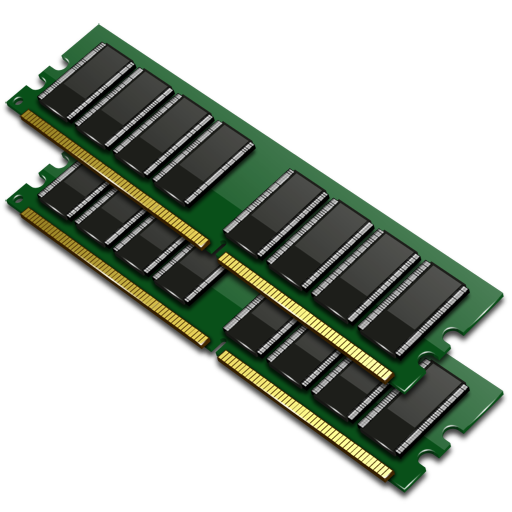
\includegraphics[width=3cm]{ram.png}
		\centering
		\caption{ram}
		\label{fig:ram}
	\end{figure}
	
	\subsection{Memoria ROM}
	Esta memoria es de tipo solo lectura y almacena datos que no pueden ser perdidos, esta memoria es importante para el arranque del programa inicial del sistema. \cite{TecnologiaInformatica}
	
	A continuación se presenta figura de una memoria ROM tomada de freepng.es (\ref{fig:rom})
	\begin{figure}[h]
		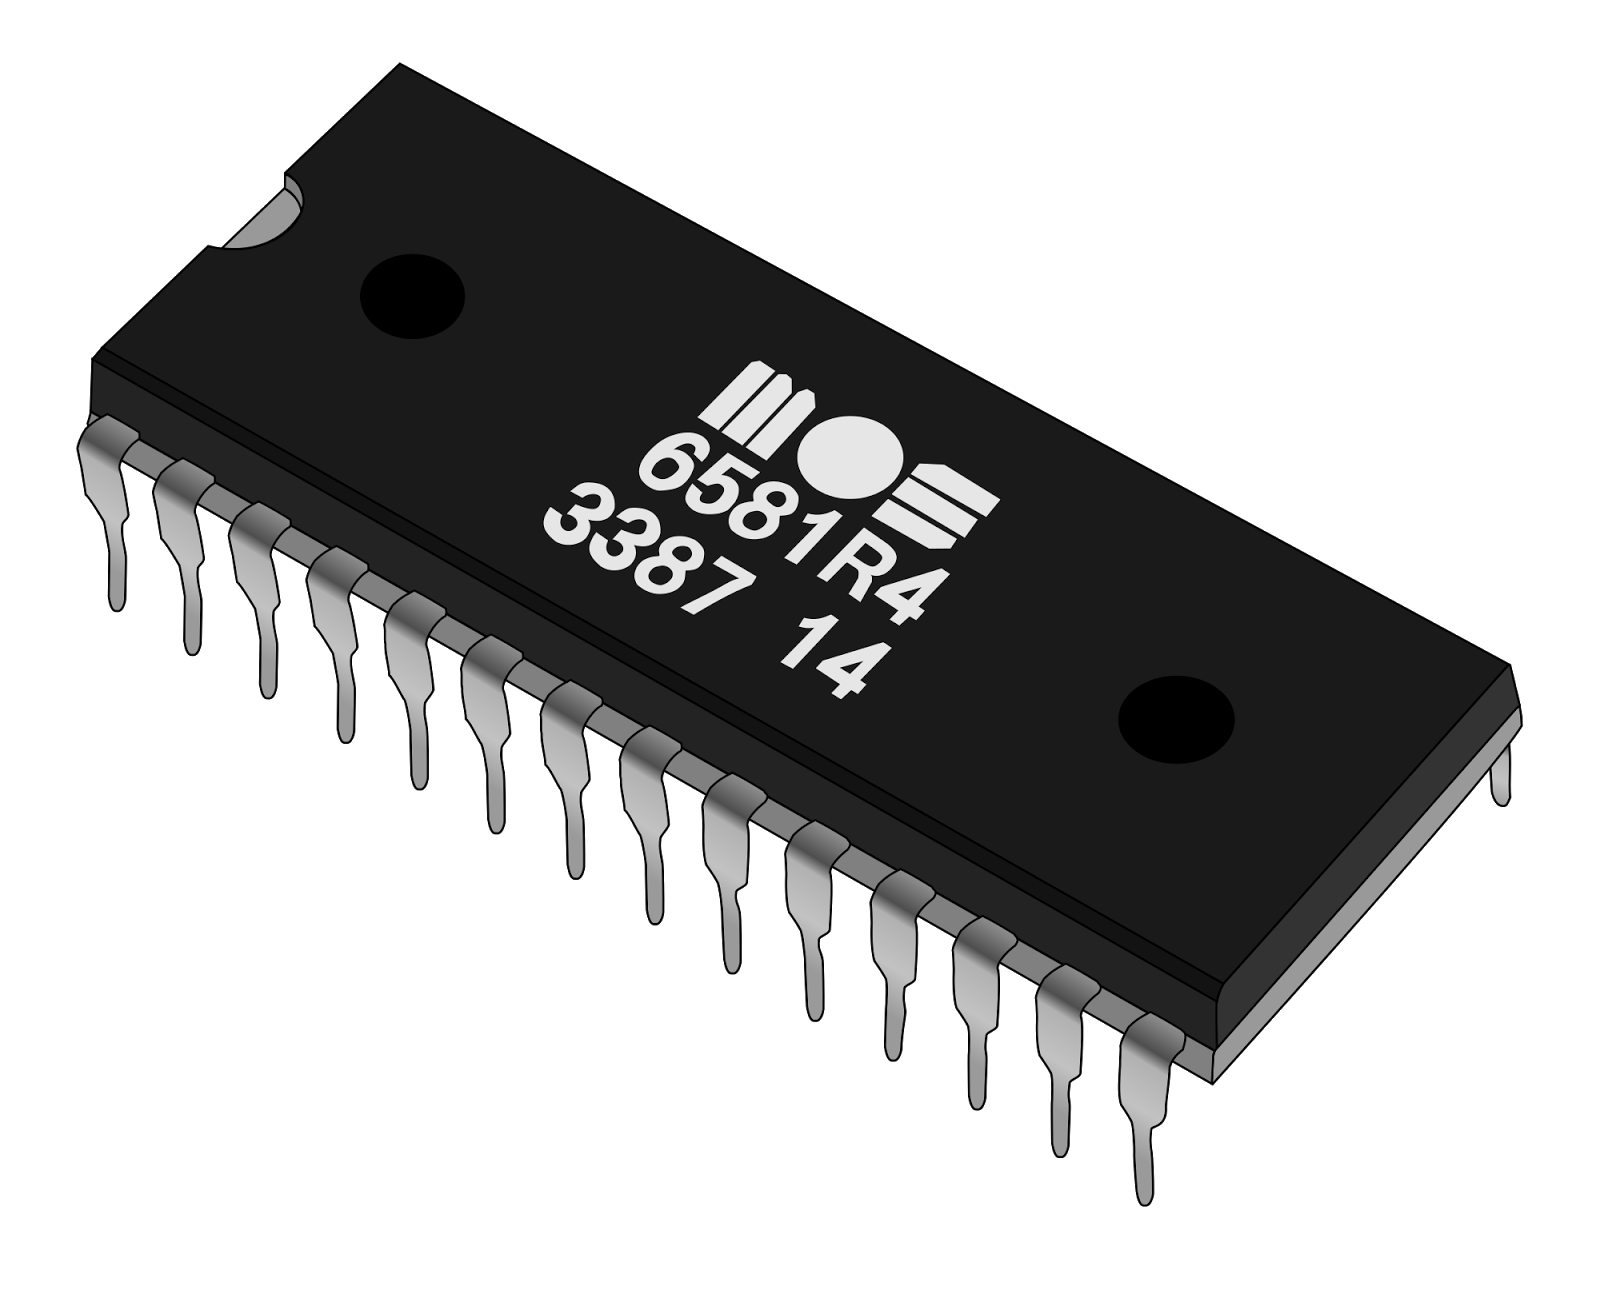
\includegraphics[width=3cm]{rom.png}
		\centering
		\caption{rom}
		\label{fig:rom}
	\end{figure}
	\subsection{Disco duro}
	El disco duro es una memoria secundaria no volátil que nos permite almacenar todo tipo de información y en grandes cantidades, el funcionamiento de este es el de almacenar la información en platos con "1", "0" o neutro de forma binaria para ser interpretada por los sistemas.\cite{TecnologiaInformatica}
	
	A continuación se presenta figura de un disco duro tomada de freepng.es(\ref{fig:hdd})
	\begin{figure}[h]
		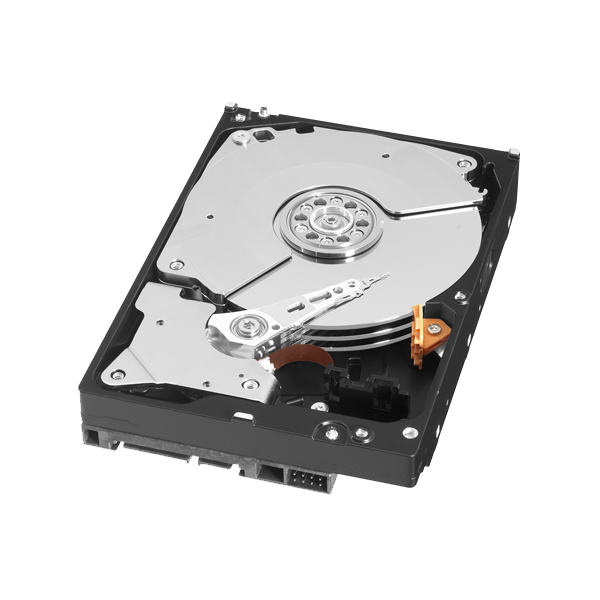
\includegraphics[width=3cm]{hdd.png}
		\centering
		\caption{hdd}
		\label{fig:hdd}
	\end{figure}
	
	\section{Gestión de la memoria del computador}
	Para dar a entender como es la gestión de la memoria del equipo de cómputo es necesario mencionar que existe una jerarquía partiendo de un registro del CPU y siguiendo dos líneas fundamentales que son el almacenamiento temporal y el almacenamiento persistente.
	\subsection{Almacenamiento temporal}
	El almacenamiento temporal esta constituido por la memoria ram, la memoria cache y la memoria virtual. La memoria cache (SRAM) es un tipo de memoria que subdivide en tres niveles de gestion que son el cache L1 que es el mas rapido, capaz de funcionar a la velocidad de los nucleos del microprocesador y a su vez el mas pequeño con respecto a la capacidad de almacenar entre los tres, después esta el cache L2 que tiene mucha mas capacidad para almacenar que el cache L1, aunque trabaje junto con los nucleos del microprocesador no es igual de rapido que el cache L1, y por ultimo esta el cache L3 que es donde queda cacheada el resto de la información. El funcionamiento de la memoria cache consiste en copiar los datos a cada uno de los niveles de cache que el microprocesador identifica como mas utilizados seguidamente de la memoria ram. Dentro de la jerarquía de la memoria sigue acontinuación la memoria principal que se refiere a la memoria ram (Random Access Memory) que no es tan rapida que la memoria cache pero cuenta con una gran capacidad de almacenamiento que le permite gestionar la mayor parte de la informacion del equipo de computo. La memoria ram esta divida en celdas que le permiten guardar bits que componen a los bytes de la información que el microprocesador necesita para su funcionamiento, ahora bien, el funcionamiento de la memoria ram consiste en guardar la información de una manera no secuencial, es decir, que la memoria ram puede acceder a la informacion de forma aleatoria, lo cual es muy rapida para ser procesada por el mismo microprocesador. Por ultimo esta la memoria virtual que es una parte del disco duro  reservada solo para guardar información que no es muy utilizada pero que deben estar lista en el momento requerido, esta memoria se manisfiesta mas cuando la memoria ram tiene cuelgues de capacidad, pero el uso de esta memoria ram puede afectar en grandes cantidades el rendimiento de nuestro equipo de computo. \cite{memorypc}
	
	\subsection{Almacenamiento persistente}
	Dentro del almacenamiento persistente encontramos memorias llamadas también memorias secundarias como la memoria ROM que guarda la información necesaria para el arranque del computador, otra memoria de esta categoría es el disco duro, el cual es el dispositivo con más capacidad de información dentro del equipo de cómputo y es donde se guarda la mayoría de datos del usuario.
	A continuación se presenta la jerarquía de la memoria(\ref{fig:Jerarquía Memoria})
	\begin{figure}[h]
		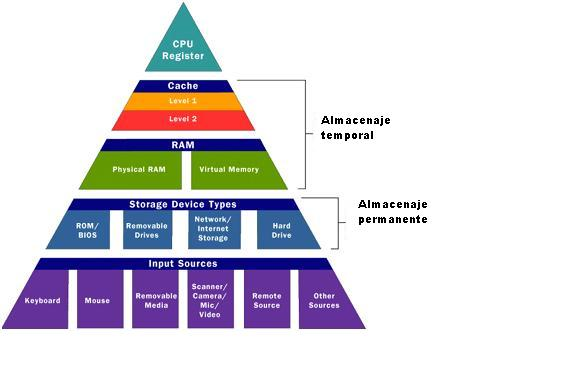
\includegraphics[width=10cm]{jq.JPG}
		\centering
		\caption{Jerarquía Memoria}
		\label{fig:Jerarquía Memoria}
	\end{figure}
	
	\section{¿Qué hace más rápida una memoria que otra memoria?}
	En lo que va del siglo se sigue necesitando de memorias que sean suficientemente rápidas y capaces para que el microprocesador funcione a su máxima potencia, por eso van surgiendo nuevas tecnologías como las memorias de Intel Optane que unifican las ventajas de la memoria RAM y el disco duro para obtener mayor velocidad y también están los discos solidos (SSD) que son más rápidos que los discos duros tradicionales, también es relacionada la velocidad con la frecuencia en que trabajan las memorias, la tasa de transferencia de nuestro disco duro pero la velocidad de las memorias también están relacionas con los buses (canales de datos) que conectan el microprocesador con la memoria RAM y la RAM con el resto de memorias, se dice que la velocidad de transferencia del bus es mucho más rápida si la memoria RAM está más cerca del microprocesador.
	\bibliographystyle{IEEEtran}
	\bibliography{references}
\end{document}
